% !TeX root = ../thuthesis-example.tex

\chapter{THE VR-IOT RESEARCH PLATFORM}

Before the platform's development, several meetings were held to discuss key implementation details and the architecture of the VR-IoT research platform, or, as it was named later, "NUIX-Studio."

Based on the first meeting discussion, it was decided that the main functions of the platform would be:
\begin{enumerate}
     \item Visualization of devices;
     \item Interaction with devices;
     \item Simulation of device sensors.
\end{enumerate}

The platform is not intended to support all types of devices. However, it must provide an API to support different ways of interaction.

After several brainstorming sessions, it was proposed to divide device controls into touch interface interaction and other ways of interaction, such as voice control. The ability to control devices at a distance, such as hand gestures, lengthening the arms, dropping hands, etc., was allocated to a separate category, possible only in virtual reality. Still, in the future, it can be implemented in the real world by the introduction of new technologies such as holographic projection.

Besides, devices can be distinguished by size, shape, various physical parameters such as sensors, lamps, non-touch screens, etc.

To preserve the narrative structure, the author introduces only the final platform prototype. However, the entire development cycle and the challenges faced are shown in Appendix.

\section{Platform requirements}
Firstly, the requirements the platform should follow are:
\begin{enumerate}
\item Scalability. The performance of the platform should stay acceptable when the number of devices in the system increases;
\item Ease of use and testing. Using Virtual Reality and IoT devices requires intuitive interaction with different kinds of elements. As for real-world devices, only sensor data collection should be implemented, while creating an API for virtual reality digital representation of devices can be a challenge. Another important task is the simulation of VR interactions on a computer for ease of testing;
\item Fault Tolerance. The platform should effectively handle faults coming from both real and virtual worlds;
\item Simultaneous work. As in the real world, where several people can interact with an IoT system at the same time, each of the platform's running instances should be able to run simultaneously and operate with the same data.
\end{enumerate}

To provide fault tolerance, the platform is based on the three layers (Figure~\ref{fig:BasicPlatformStructure-figure}): 
\begin{enumerate}
    \item Real-world IoT devices HUB. A special device responsible for receiving and sending data to real-world devices is needed, that provides the data in a unified format (abstraction of sensors).
    A third-party software openHAB (\cite{OpenHab}) is used with a future upgrade to a standalone solution to support different IoT devices. The HUB runs on a server and is responsible for collecting and storing the IoT devices' data. Managing the data is performed through a Web Interface;
    \item Integration layer. Responsible for analyzing data coming from VR and real-world, integrating real-world devices data into VR and vice-versa, performing persistence and providing API for using the platform in research projects. By receiving and sending unified data objects representing IoT devices' sensor data using REST API calls, each of the NUIX-Studio App instances operates with the same data, enabling simultaneous work. The next step is to represent IoT devices' data in Virtual reality and perform computations for research. Since the platform should run smoothly on VR headsets and provide good UX, the analysis should be performed on a PC\footnote{In Chapter 4 an experiment proving this statement is provided.}. At the same time, Virtual reality headsets perform computations for interacting with objects, such as hand recognition. 
    \item Visualization layer. Interaction with digital IoT devices can be performed using VR headsets, AR devices, or simulating touch, sight, gestures, and other interactions. The platform provides an API for developers to integrate their interaction techniques into this layer, but developing these techniques is not the focus of this research. It was decided to use Unity (\cite{Unity}) for interaction with virtual reality devices. Firstly, Unity comes with a ready-to-use 3D engine, relieving the need to develop a new one. Secondly, Unity is multi-platform and supports VR headsets. Thirdly, developers are already familiar with Unity development, making it easier for them to integrate the platform into their solutions.
\end{enumerate}

\begin{figure}
  \centering
  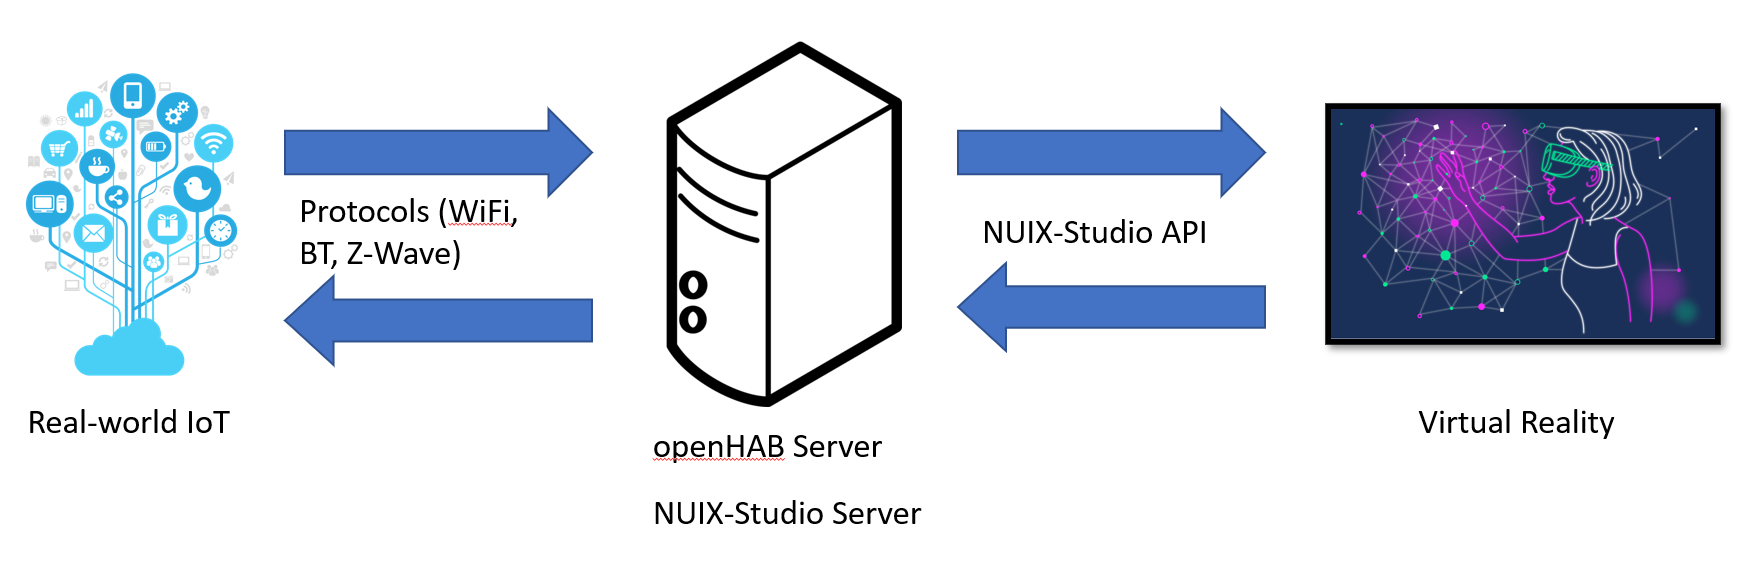
\includegraphics[width=0.9\linewidth]{figures/BasicPlatformStructure.png}
  \caption{Simplified structure of NUIX Studio. Real-world IoT devices HUB is an openHAB server, while NUIX-Studio server is an instance of NUIX-Studio APP responsible for the computations.}
  \label{fig:BasicPlatformStructure-figure}
\end{figure}

\section{Server Architecture}
\subsection{OpenHAB Server Structure}

It was decided not to change the openHAB system's structure since it follows the SOA principles that allow implementing support for various types of devices (Figure~\ref{fig:BasicPlatformStructure-figure}).

Each IoT device is called a Thing, but a Thing can also be a service. For example, a smoke sensor and user location are both Things.

Things expose their capabilities through Channels. For example, smart vacuum cleaner channels can be suction strength, water delivery strength, remaining charge level, and cleaning status.

Each channel is associated with one or more Items that are added inside the model. Items have a State, and they may receive commands. 

Before adding an IoT device to the server, the developer has to install a software adapter first. These add-ons are called bindings, and they provide a way to link Items to physical devices.

\begin{figure}
  \centering
  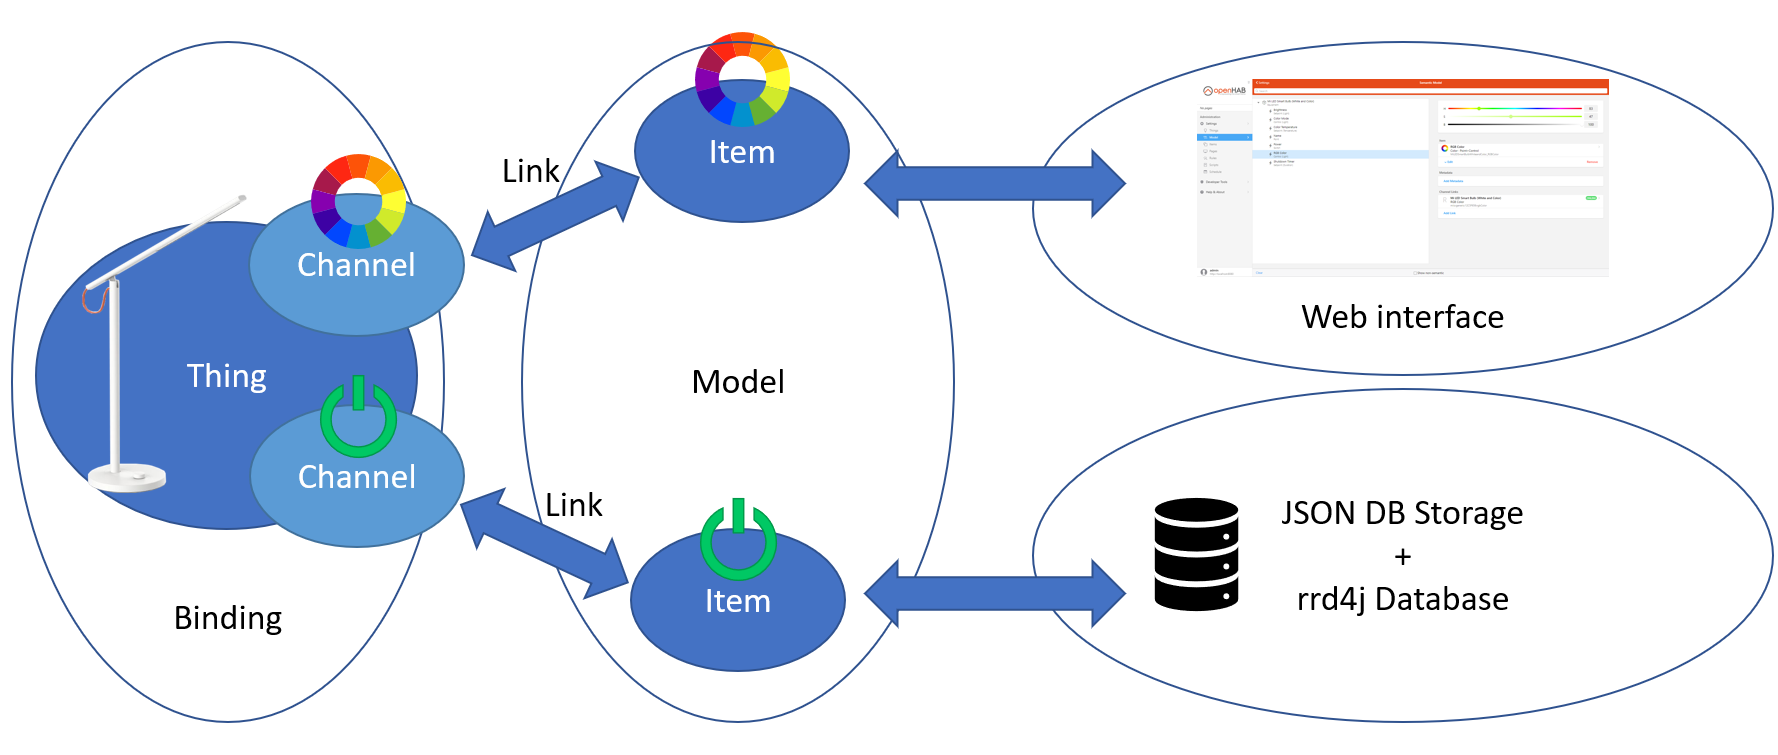
\includegraphics[width=0.9\linewidth]{figures/openHABServerStructure.png}
  \caption{Server structure}
  \label{fig:openHABServerStructure-figure}
\end{figure}

In the example, each of the items is linked to only one channel, and each of the channels is linked to only one item. 

When a binding for Xiaomi smart home devices is installed, the smart home devices can be automatically discovered by the server and added as Things. A Xiaomi Lamp is used in the example, for which several Channels are presented (Figure~\ref{fig:XiaomiLampChannels-figure}).

\begin{figure}
  \centering
  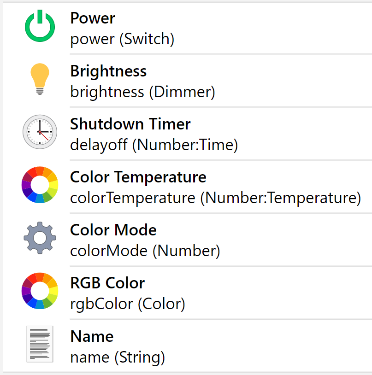
\includegraphics[width=0.6\linewidth]{figures/XiaomiLampChannels.png}
  \caption{Channels list example.}
  \label{fig:XiaomiLampChannels-figure}
\end{figure}

Each of these channels represents one item (Figure~\ref{fig:XiaomiLampPowerItem-figure}).

\begin{figure}
  \centering
  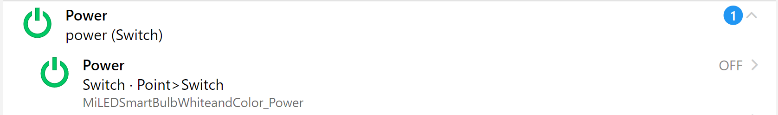
\includegraphics[width=0.9\linewidth]{figures/XiaomiLampPowerItem.png}
  \caption{An Item example.}
  \label{fig:XiaomiLampPowerItem-figure}
\end{figure}

For example, the Power Control is performed through the power channel. In terms of the introduced concepts, the Power Control is an Item named MiLEDSmartBulbWhiteandColorPower of type Switch and State "OFF."

As soon as the lamp is turned On, the Power Control switch in Web Interface will also turn ON. And if the switch is changed to the "OFF" state in the Web Interface, the lamp will turn off.

To support Fault Tolerance, the openHAB server stores data over time.

\subsection{Server Extended Structure}

In the previous section, it was not specified how the platform should perform access to the server data. 

\begin{figure}
  \centering
  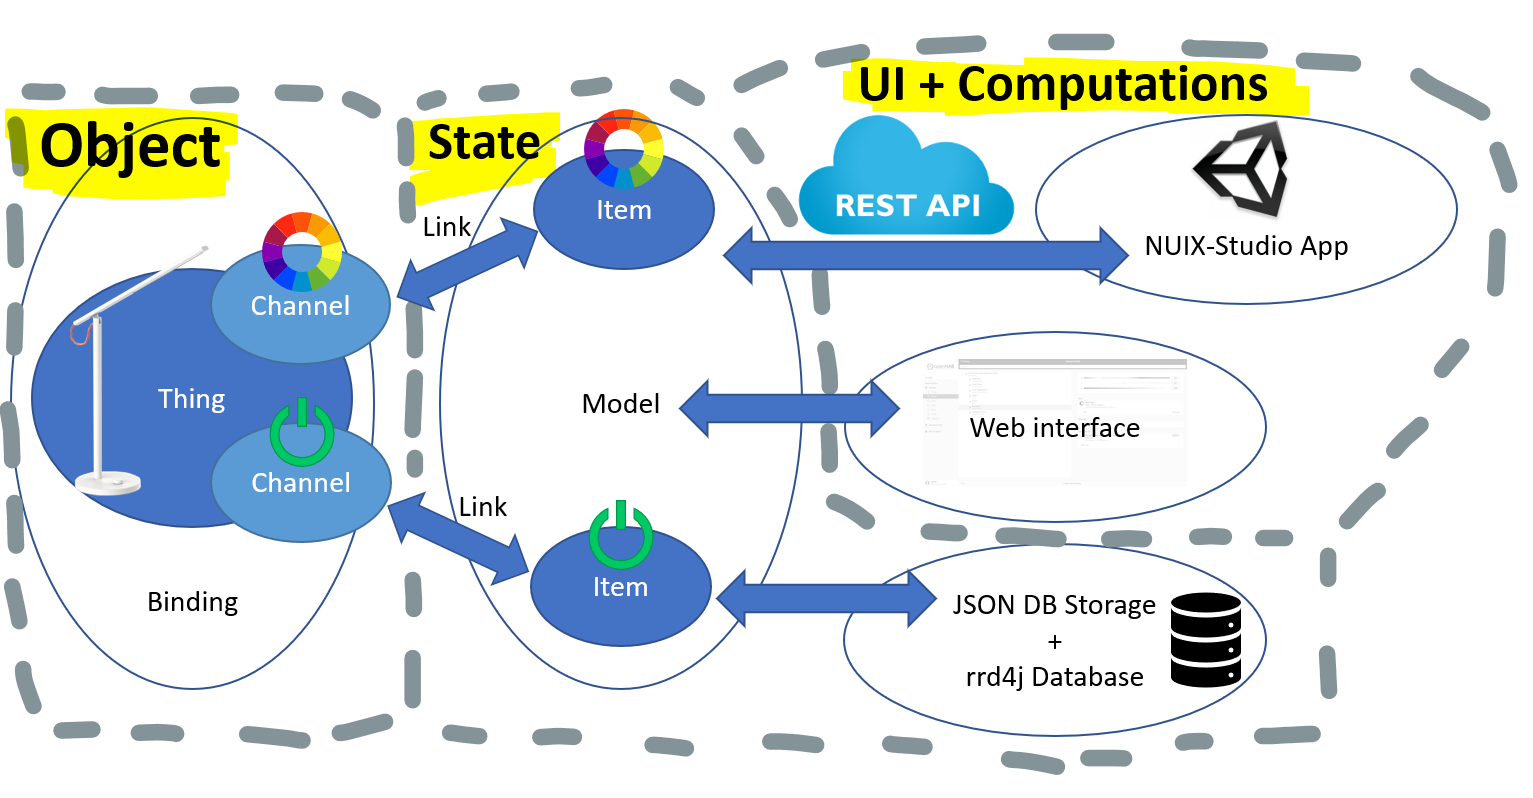
\includegraphics[width=0.9\linewidth]{figures/ExtendedServerStructure.png}
  \caption{Structure of the server showing how the NUIX-Studio APP is connected to it.}
  \label{fig:ExtendedServerStructure-figure}
\end{figure}

Syncing is performed through REST API (Table~\ref{tab:rest-api-table}), which is explained in detail further.

\begin{table}
  \centering
  \begin{threeparttable}[c]
    \caption{REST API commands used in NUIX-Studio}
    \label{tab:rest-api-table}
    \begin{tabular}{ll}
      \toprule
      REST API CALL    &         DESCRIPTION                 \\
      \midrule
      GET\tnote{a} & Get all available items \\
      POST\tnote{b} & Adds a new item to the registry or updates the existing item    \\
      PUT\tnote{b}        & Sends a command to the item                              \\
      DELETE\tnote{b}        & Removes an item from the registry          \\
      \bottomrule
    \end{tabular}
    \begin{tablenotes}
      \item [a] For link: /items
      \item [b] For link: /items/<itemname>
    \end{tablenotes}
  \end{threeparttable}
\end{table}

In the current implementation of the platform, four different REST API commands are used: GET command for receiving the items in the registry on system startup, PUT command to create a new item on the server, POST command for updating the state of the item, and DELETE command for removing an item from the server.

States of the items are received by getting the events from the server: once the event is received, the item state can be retrieved from the payload.

\section{NUIX-Studio App}

As mentioned above, there can be several NUIX-Studio APP instances running at the same time. Each of them has access to the Server through REST API. The instances can be of one of three types:

\begin{enumerate}
    \item Virtual Reality Instance. It runs on Oculus or another VR headset, has remote or local access to the server. Items received from the server are visualized. It is possible to interact with the items in different ways such as touching buttons, moving sliders, performing hand gestures, using voice commands, etc. 
    \item Computations Instance. It runs on a powerful machine and has either remote or local access to the server. Since latency is important for the VR-IoT platform, it is preferable to run this instance on the same machine as openHAB. In this case, the REST API calls time will be less than the minimum measurement unit (compared to milliseconds for accessing remote virtual reality instances)\footnote{An experiment to prove this statement is provided in Chapter 4.}. Physics, Big Data analysis, and other performance-based computations are executed in this instance, while user interactions are limited.
    \item Input simulation instance. If the APP instance runs on the device with limited support of interaction interfaces (for example, a PC), input simulation can be used. Sometimes, it is even easier to run and test the platform on such devices: for example, if using a physical keyboard is required or when there is no access to a VR headset.
\end{enumerate}

\begin{figure}
  \centering
  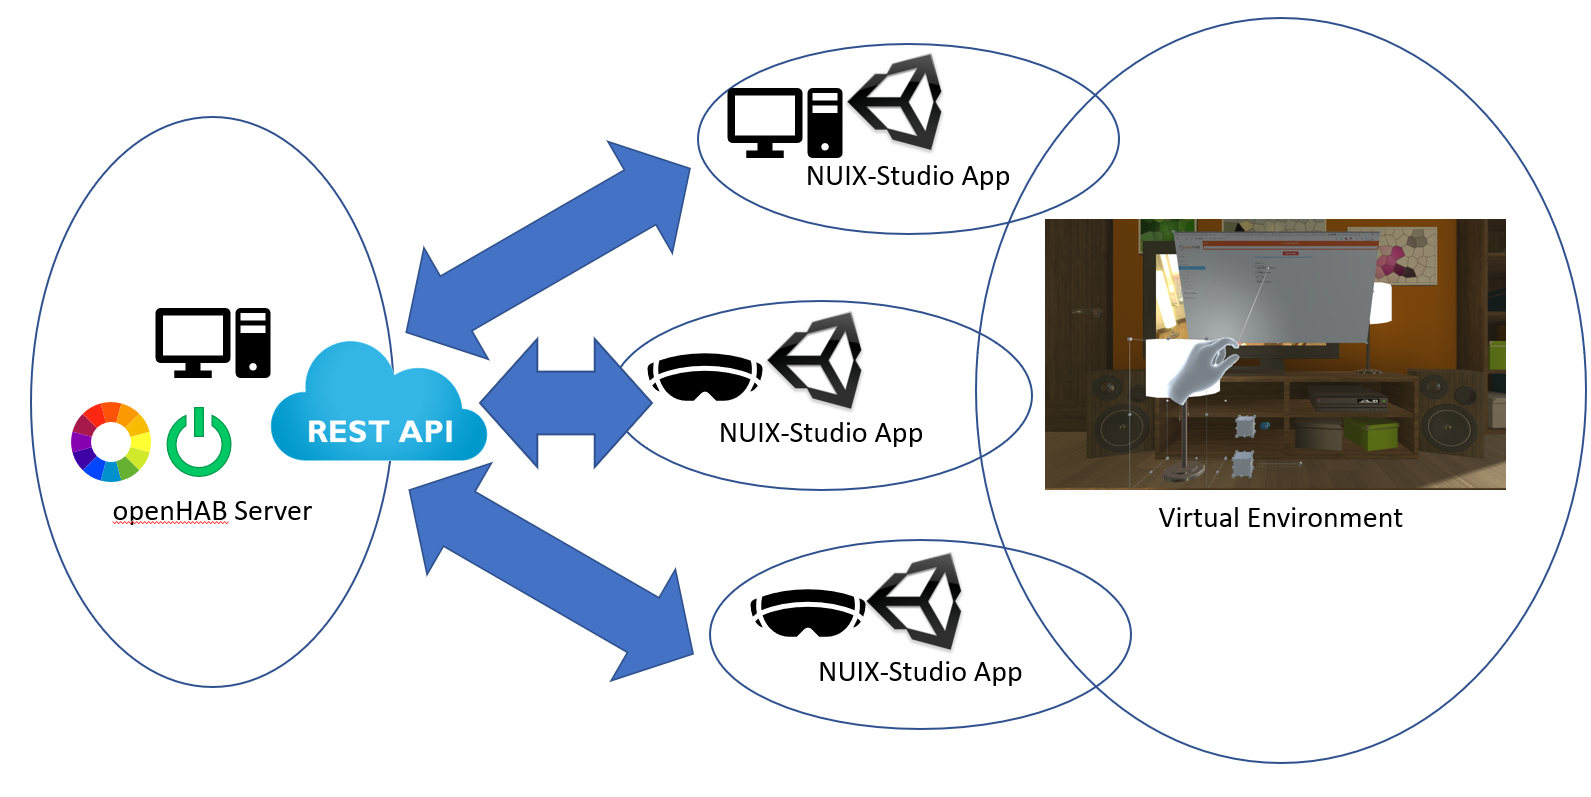
\includegraphics[width=0.9\linewidth]{figures/AppInstances.png}
  \caption{NUIX-Studio App Instances}
  \label{fig:AppInstances-figure}
\end{figure}

Each of the instances has access to the same data on the server, making it possible to work simultaneously in one virtual environment and divide tasks between several NUIX-Studio App instances (Figure~\ref{fig:AppInstances-figure}). One of the instances can be used for computations, while others can be used for interacting with the devices in Virtual reality.

\subsection{NUIX-Studio App Architecture}

When the NUIX-Studio APP requests access to the system to get the list of items from the registry, a list of Item Data Transfer Objects is received by the app and then added into Semantic Model (Figure~\ref{fig:AppArchitecture-figure}). When the state of the item is updated, or if a an item is added or removed, an event is sent to the EventController instance, and then, based on the event payload, the item list is updated.  Keeping each item's data equal to the server's, the Semantic model in NUIX-Studio APP is equivalent to the Semantic model presented on the server. 

But storing the states of the items in the APP by itself does not allow user to interact with the items. In other words, NUIX-Studio App has to provide an interface to interact with the items. Since different types of items require different interaction techniques, for each item type, a widget is created.
Widget in NUIX-Studio APP is a Unity Virtual GameObject, which can visualize the item state and update it. For example, it can be an interactable pinch slider for a dimmer item or a virtual screen for an image item.

By integrating Extra packages, NUIX-Studio platform can provide a bigger variety of widgets and a higher number of supported devices. For example, Oculus Integration support provides an API for hands recognition; SteamVR (\cite{SteamVR2021}) support makes it possible to run the NUIX-Studio APP on the majority of VR headsets.

\begin{figure}
  \centering
  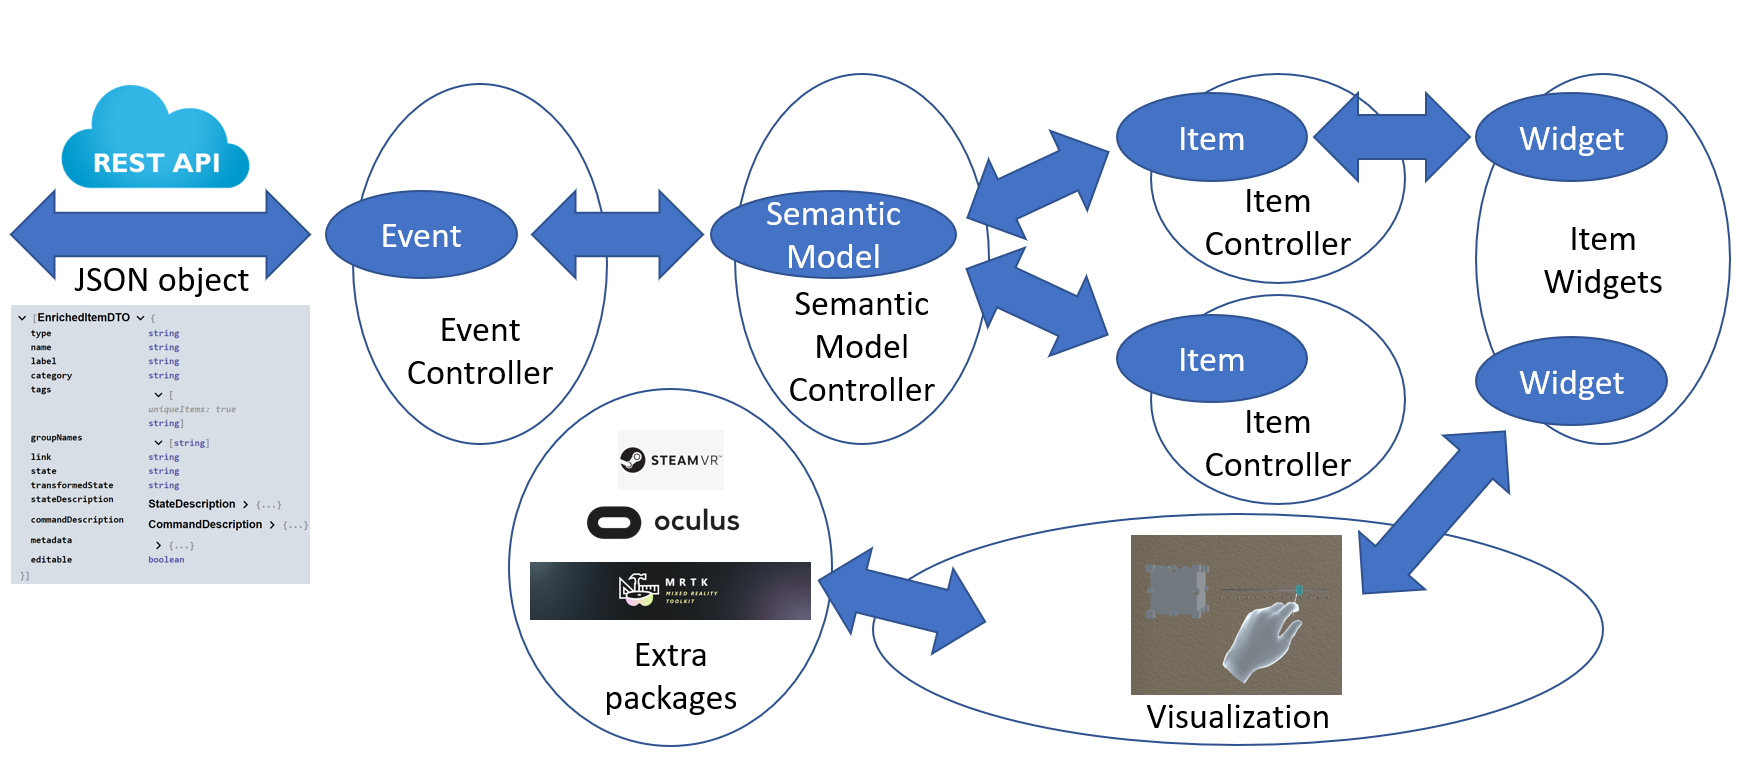
\includegraphics[width=0.9\linewidth]{figures/AppArchitecture.png}
  \caption{NUIX-Studio App Architecture}
  \label{fig:AppArchitecture-figure}
\end{figure}

\subsection{NUIX-Studio App Semantic Model}

As mentioned above, the Semantic model in the NUIX-Studio App is kept equivalent to the Semantic model stored on the server. The advantages of this approach are listed below:

\begin{enumerate}
    \item Each of the APP instances visualizes equivalent data, providing simultaneous and fault-tolerance work;
    \item The Semantic model on the server is time and memory-effective.
\end{enumerate}

Overall, using the defined approach, the platform follows the Dependency-inversion principle "depend upon abstractions, not concretions."(TODO: add reference to this citation) In this case, the Semantic model is an abstraction, and Item representation is an abstraction as well.

But when it is required to provide an interface for creating new IoT devices in VR and interaction with them, it is not possible to use items presented on the server only. For example, each item's virtual position is a required data, which should be accessible by each of the instances.

Therefore, the disadvantages of keeping the fully equivalent Semantic models are explained below:

\begin{enumerate}
    \item The Semantic model should be extended with extra items, such as virtual position or environment setup. These items are needed by each running instance of the NUIX-Studio APP.
    \item The platform's main purpose is to provide an interface to test new IoT devices inside Virtual reality or extend the existing items with extra functionality. But only real-world devices' data is stored on the server.
\end{enumerate}

As a result, extending the Semantic model with virtual items helps to minimize the number of disadvantages while keeping the advantages.
In the next Chapter, an example of using the NUIX-Studio is given, and the measured performance is analyzed.